\documentclass[11pt,letterpaper]{article}

\usepackage[utf8]{inputenc}
\usepackage[spanish,es-nodecimaldot]{babel}
\usepackage{amsmath}
\usepackage{amssymb}

\usepackage{tabu}

\usepackage[most]{tcolorbox}
\usepackage{multicol}

\usepackage{mathtools}
\usepackage{tikz}

\usepackage[top=1in, bottom=1in, left=1in, right=1in]{geometry}


\begin{document}

\begin{titlepage}
    \centering

    {\scshape\LARGE Universidad Nacional Autónoma de México \par}

    \vspace{1cm}
    {\scshape\Large Facultad de Ciencias\par}
    \vspace{1.5cm}

    \begin{center}
        
\includegraphics[scale=.1]{../../assets/img/logo.png}
    \end{center}

    \vspace{.8 cm}

    {\LARGE Tarea semanal 09: \par}
    {\huge\bfseries Relaciones y gráficas \par}

    \vspace{0.5cm}
    {\large\itshape Pablo A. Trinidad Paz\par}
    419004279

    \vfill

    Trabajo presentado como parte del curso de \textbf{Estructuras Discretas}
    impartido por la profesora \textbf{Pilar Selene Linares Arévalo}. \par
    \vspace{0.1cm}
    {\large 23 de Noviembre de 2018\par}
\end{titlepage}

\begin{enumerate}

    \item Decide cuáles de las propiedades, reflexiva, simétrica, transitiva o antisimétrica,
    cumplen las siguientes relaciones $R$ y $S$ (representadas por las gráficas de abajo). Justifica.

        \begin{center}
            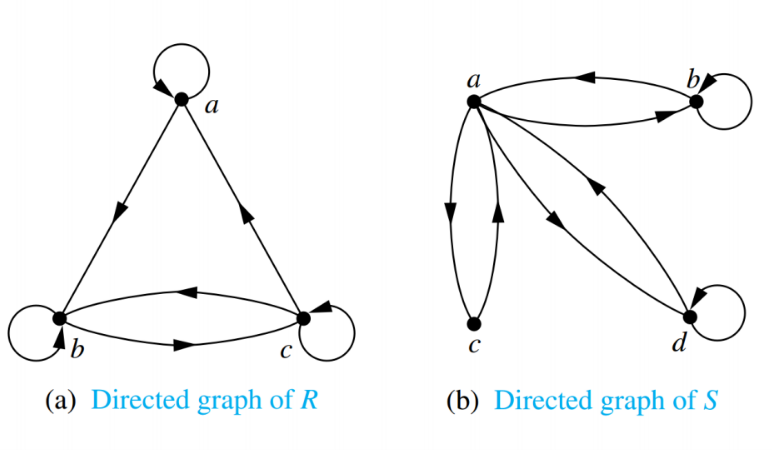
\includegraphics[scale=.3]{assets/graphs.png}
        \end{center}

        \textbf{Solución: } Las gráficas $R$ y $S$ pueden ser representados como:

        \begin{equation*} \begin{split} \begin{aligned}
            R &= {(a,a), (a,b), (b,b), (b,c), (c,c), (c,b), (c, a)} \\
            S &= {(a, b), (a, c), (a, d), (b, b), (b,a), (c, a), (d, d), (d, a)} \\
        \end{aligned} \end{split} \end{equation*}

        $R \subseteq A \times A$ donde $A = \{a, b, c\}$:
        \begin{itemize}
            \item \textbf{Es reflexiva} porque $\forall a \in A, (a, a) \in R$
            \item \textbf{NO es simétrica} porque $\{(a, b),(c, a)\} \subset R$ pero $\{(b, a), (a, c)\} \not\subset R$
            \item \textbf{NO es transitiva} porque $\{(a,b), (b, c)\} \subset R$ pero $\{(a, c)\} \not\subset R$
            \item \textbf{NO es antisimétrica} porque $\{(b, c), (c, b)\} \subset R$ pero $b \neq c$
        \end{itemize}

        $S \subseteq B \times B$ donde $B = \{a, b, c, d\}$:
        \begin{itemize}
            \item \textbf{NO es reflexiva} porque no se cumple que $\forall a \in B, (a, a) \in S$
            \item \textbf{Es simétrica} porque $\forall a, b \in B$, sucede que si $(a, b) \in S$, entonces $(b, a) \in S$
            \item \textbf{NO es transitiva} porque $\{(a, b), (b, a)\} \subset S$ pero $\{(a, a)\} \not\subset S$
            \item \textbf{NO es antisimétrica} porque $\{(a, b), (b, a)\} \subset S$ pero $a \neq b$
        \end{itemize}

    \clearpage
    \item Considera las siguientes matrices de las relaciones $R_1, R_2 \subseteq A \times A$ con $A = \{a, b, c\}$:
        \begin{equation*} \begin{split} \begin{gathered}
            R_1 = \begin{bmatrix}
                1 & 0 & 1 \\
                0 & 1 & 0 \\
                1 & 0 & 1
            \end{bmatrix} \qquad
            R_2 = \begin{bmatrix}
                1 & 0 & 0 \\
                1 & 0 & 0 \\
                1 & 1 & 1
            \end{bmatrix}
        \end{gathered} \end{split} \end{equation*} \\

        \begin{enumerate}
            \begin{multicols}{4}
                \item Calcula $R_1 \cup R_2$
                    \begin{equation*} \begin{split} \begin{gathered}
                        \begin{bmatrix}
                            1 & 0 & 1 \\
                            1 & 1 & 0 \\
                            1 & 1 & 1
                        \end{bmatrix}
                    \end{gathered} \end{split} \end{equation*}
                \item Calcula $R_1 \cap R_2$
                    \begin{equation*} \begin{split} \begin{gathered}
                        \begin{bmatrix}
                            1 & 0 & 0 \\
                            0 & 0 & 0 \\
                            1 & 0 & 1
                        \end{bmatrix}
                    \end{gathered} \end{split} \end{equation*}
                \item Calcula $R_1 - R_2$
                    \begin{equation*} \begin{split} \begin{gathered}
                        \begin{bmatrix}
                            0 & 0 & 1 \\
                            0 & 1 & 0 \\
                            0 & 0 & 0
                        \end{bmatrix}
                    \end{gathered} \end{split} \end{equation*}
                \item Calcula $R_1^c$
                    \begin{equation*} \begin{split} \begin{gathered}
                        \begin{bmatrix}
                            0 & 1 & 0 \\
                            1 & 0 & 1 \\
                            0 & 1 & 0
                        \end{bmatrix}
                    \end{gathered} \end{split} \end{equation*}
                \item Calcula $R_2^{-1}$
                    \begin{equation*} \begin{split} \begin{gathered}
                        \begin{bmatrix}
                            1 & 1 & 1 \\
                            0 & 0 & 1 \\
                            0 & 0 & 1
                        \end{bmatrix}
                    \end{gathered} \end{split} \end{equation*}

                \item Calcula $R_2 \cdot R_1$
                    \begin{equation*} \begin{split} \begin{gathered}
                        \begin{bmatrix}
                            1 & 0 & 1 \\
                            1 & 0 & 1 \\
                            1 & 1 & 1
                        \end{bmatrix}
                    \end{gathered} \end{split} \end{equation*}

                \item Calcula $R_1 \cdot R_2$
                    \begin{equation*} \begin{split} \begin{gathered}
                        \begin{bmatrix}
                            1 & 0 & 1 \\
                            1 & 0 & 1 \\
                            1 & 1 & 1
                        \end{bmatrix}
                    \end{gathered} \end{split} \end{equation*}
            \end{multicols}
        \end{enumerate}

\end{enumerate}

\end{document}
